% IEEE standard conference template; to be used with:
%   spconf.sty  - LaTeX style file, and
%   IEEEbib.bst - IEEE bibliography style file.
% --------------------------------------------------------------------------

\documentclass[letterpaper]{article}
\usepackage{spconf,amsmath,amssymb,graphicx}
\usepackage{hyperref,url}

\usepackage{graphicx}
\usepackage[x11names, rgb]{xcolor}
\usepackage[figuresright]{rotating}
\usepackage{pgfplots}
\usepackage{tikz}
\pgfplotsset{compat=1.10}
\usepgfplotslibrary{fillbetween}
\usetikzlibrary{snakes,arrows,shapes,plotmarks,calc}

\newcommand\Top{\rule{0pt}{3ex}}
\newcommand\Bot{\rule[-1.5ex]{0pt}{0pt}}

% Monokai colors
\definecolor{color0}{HTML}{272822}
\definecolor{color1}{HTML}{383830}
\definecolor{color2}{HTML}{49483E}
\definecolor{color3}{HTML}{75715E}
\definecolor{color4}{HTML}{A59F85}
\definecolor{color5}{HTML}{F8F8F2}
\definecolor{color6}{HTML}{F5F4F1}
\definecolor{color7}{HTML}{F9F8F5}
\definecolor{color8}{HTML}{F92672}
\definecolor{color9}{HTML}{FD971F}
\definecolor{color10}{HTML}{F4BF75}
\definecolor{color11}{HTML}{A6E22E}
\definecolor{color12}{HTML}{A1EFE4}
\definecolor{color13}{HTML}{66D9EF}
\definecolor{color14}{HTML}{AE81FF}
\definecolor{color15}{HTML}{CC6633}
\newcommand\showcolors{
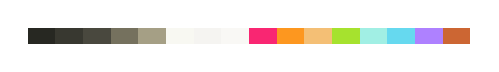
\begin{tikzpicture}
  \foreach \pos/\col in {0em/color0, 1em/color1, 2em/color2, 3em/color3, 
  4em/color4, 5em/color5, 6em/color6, 7em/color7, 8em/color8, 9em/color9, 
  10em/color10, 11em/color11, 12em/color12, 13em/color13, 14em/color14, 
  15em/color15}
  \fill[\col] (\pos,0) rectangle +(1em, 0.6em);
\end{tikzpicture}
}

% Example definitions.
% --------------------
% nice symbols for real and complex numbers
\newcommand{\R}[0]{\mathbb{R}}
\newcommand{\C}[0]{\mathbb{C}}

% bold paragraph titles
\newcommand{\mypar}[1]{{\bf #1.}}

% Title.
% ------
\title{Parallel build of randomized k-d trees and fast approximate kNN search on Xeon Phi}
%
% Single address.
% ---------------
% \name{Markus P\"uschel\thanks{The author thanks Jelena Kovacevic. This paper
% is a modified version of the template she used in her class.}} 
% \address{Department of Computer Science\\ ETH Z\"urich\\Z\"urich, Switzerland}

% For example:
% ------------
%\address{School\\
%		 Department\\
%		 Address}
%
% Two addresses (uncomment and modify for two-address case).
% ----------------------------------------------------------
\twoauthors%
{P. Santhanam\sthanks{psanthan@student.ethz.ch}, J. C. de Fine 
Licht\sthanks{definelj@student.ethz.ch}}%
{ETH Z\"urich\\%
Department of Computer Science\\%
Universit\"atstrasse 6, 8006 Z\"urich}%
{F. Wermelinger\sthanks{fabianw@mavt.ethz.ch}}%
{ETH Z\"urich\\%
% Computational Science and Engineering Laboratory\\%
Chair of Computational Science\\%
Clausiusstrasse 33, 8092 Z\"urich}%

\begin{document}
%\ninept
\maketitle

\begin{abstract}
  We present a parallel $k$-nearest neighbor search algorithm ($k$-NN) for 
  large datasets of high dimensionality.  A $k$-NN algorithm is used for image 
  classification, simulations of particles with a large number of attributes, 
  regression problems as well as other applications.  Depending on the size of 
  the input, a search of a linear data structure can be computationally 
  expensive.  We use randomized k-d~trees as an accelerating structure of high 
  dimensional data to improve search performance.   Our work is focused on the 
  parallel build of randomized k-d~trees using the Intel threading building 
  blocks library (TBB), as well as improving search performance using the Intel 
  XeonPhi co-processor.  We compare our results against the fast library for 
  approximate nearest neighbor search (FLANN) and observe an improvement of 
  $11\times$ on two $12$-core Intel Xeon E5-2697v2 CPUs on a node of the ETH 
  Euler cluster for building the randomized k-d~trees compared against FLANN.  

  % add stuff here for the search performance? Can do but should conclude with 
  % the performance modeling?

  % Nearest neighbor search across huge amount of data with high dimensionally 
  % finds its applications in image recognition (To Do: Other Applications).  
  % These applications demand the retrieval of k-nearest neighbours to be faster.  
  % KD Tree is an accelerating data structure which can perform the search faster 
  % on the low dimensional big data set. Performance of kd tree drops to that of 
  % the linear search when it is applied for high dimensional data. By inducing 
  % approximation over the retrieved search results randomised KD trees can 
  % perform the nearest neighbour look ups faster even over the high dimensional 
  % data. KD Trees and Randomised KD trees involve a build phase overhead. This 
  % might even be a bigger problem if the input data changes frequently and we 
  % need to build the Randomised KD forest in real time.( TO DO: Abstract of How 
  % do we parallelise and etc..)
  \end{abstract}

  % Mainbody
  \section{Introduction}
  \label{sec:intro}

  % Do not start the introduction with the abstract or a slightly modified
  % version. It follows a possible structure of the introduction. 
  % Note that the structure can be modified, but the
  % content should be the same. Introduction and abstract should fill at most the first page, better less.

  \mypar{Motivation} In many applications, efficient search algorithms are of 
  great importance due to their high computational cost.  A common search 
  operation is to find a closest neighbor given some query point, which is 
  referred to as \emph{nearest neighbor search}.  This operation can readily be 
  extended to find the set of the $k$-nearest neighbors instead of just the 
  closest nearest neighbor.  The search space is usually very large and each 
  data point in such a set can be of high dimensionality.  For example, 
  matching images using distinct local image features~\cite{lowe2004a} is 
  a common task performed by web-search engines or in image recognition using 
  large datasets of up to $80$~million small images~\cite{torralba2008a}, where 
  each of the images is a high dimensional data point, depending on the number 
  of pixels used to represent the image.

  In order to speed-up the basic linear traversal of the data during the 
  search, accelerating data structures are employed.  For example, the k-d tree 
  is a simple space partitioning data structure~\cite{bentley1975a,friedman1977a}, where at each level a particular axis among the $k$ dimensions is chosen to split the points in the space.  However, exact 
  nearest neighbor search using a k-d tree is only efficient for low dimensional 
  data~\cite{muja2009a}.  For high dimensional data approximate structures, 
  such as a randomized k-d tree~\cite{silpa2008a} or hierarchical $k$-means 
  tree~\cite{muja2009a}, are used at the cost of the accuracy of the returned 
  nearest neighbors.

  In contrast to the naive linear search, an additional overhead is created by 
  building the accelerating data structure before performing the search.  
  Hence, the overall search time is composed of a build time for the data 
  structure and the time to perform the search using the structure.  Naturally, 
  the build time for a linear search vanishes.

  In this work, we focus on the fast parallel build of a set of randomized 
  k-d trees used to perform a parallel $k$-nearest neighbor search on high 
  dimensional data.  For our parallel application, we utilize the Intel many 
  integrated core (MIC) architecture offered by the Intel Knights Corner (KNC) 
  co-processor family.

  % \mypar{Motivation} The first task is to motivate what you do.  You can
  % start general and zoom in one the specific problem you consider.  In
  % the process you should have explained to the reader: what you are doing,
  % why you are doing, why it is important (order is usually reversed).

  % For example, if my result is the fastest sorting implementation ever, one
  % could roughly go as follows. First explain why sorting is important
  % (used everywhere with a few examples) and why performance matters (large datasets,
  % realtime). Then explain that fast implementations are very hard and
  % expensive to get (memory hierarchy, vector, parallel). 

  % Now you state what you do in this paper. In our example: 
  % presenting a sorting implementation that is
  % faster for some sizes as all the other ones.

  \mypar{Related work} Silpa-Anan and Hartley~\cite{silpa2008a} have proposed 
  a k-d tree algorithm based on creating multiple randomized k-d trees, where 
  each of the randomized trees splits the data based on a random choice of the 
  $D$ dimensions with highest variance.  Muja and Lowe have developed a C++ 
  library\footnote{\url{http://www.cs.ubc.ca/research/flann/}} for fast 
  approximate nearest neighbor searches with automatic algorithm selection 
  based on the data used for the search~\cite{muja2009a,muja2014a}.  The same 
  library implements a parallel build of a k-d tree for $3$D~data using GPU 
  hardware.  Building trees for high dimensional data is not parallelized.  The 
  work of Garcia~et~al.\@ employ GPUs to perform basic linear $k$-nearest 
  neighbor searches by using optimized linear algebra libraries and sorting 
  algorithms~\cite{garcia2008a,garcia2010a}.

  % \mypar{Related work} Next, you have to give a brief overview of
  % related work. For a report like this, anywhere between 2 and 8
  % references. Briefly explain what they do. In the end contrast to what
  % you do to make now precisely clear what your contribution is.

  % mainfile: ./../report.tex

  \section{$k$-Nearest Neighbor Search Algorithm}
  \label{sec:_k_nearest_neighbor_search_algorithm}

  In this section we formally define the $k$-nearest neighbor search problem 
  and introduce the... add on here

  \mypar{Nearest neighbor search} Consider a set of points $\mathcal{P} 
  = \{p_1,p_2,\dots,p_n\}$ in a metric space $\mathbb{M}$ which defines some 
  distance function $d\colon\mathbb{M}\times\mathbb{M}\to\mathbb{R}$.  If we 
  are given a query point $q\in\mathcal{P}$, the nearest neighbor of $q$ must 
  satisfy the condition
  \begin{align}
    \label{eq:NN}
    \operatorname{NN}(q,\mathcal{P}) &= \operatorname{argmin}_{x\in\mathcal{P}} 
    d(q,x)\in\mathcal{P}.
  \end{align}

  Often we are not interested in only one nearest neighbor, but the $k$~nearest 
  neighbors, for which we use the notation
  \begin{align}
    \label{eq:kNN}
    \operatorname{kNN}(q,\mathcal{P},k) &= \mathcal{A},
  \end{align}
  where $\mathcal{A}\subseteq\mathcal{P}$ with cardinality 
  $\vert\mathcal{A}\vert = k$.  The following constraint must further be 
  satisfied
  \begin{align}
    \label{eq:constraint_kNN}
    \{d(q,x)\mid d(q,x)\leq d(q,y)\forall x\in\mathcal{A}, 
    y\in\mathcal{P}-\mathcal{A},q\in\mathcal{P}\}.
  \end{align}
  Since the cardinality of $\mathcal{A}$ is $k$, it follows that $n\geq k$ for 
  the number of points in $\mathcal{P}$.

  % Give a short, self-contained summary of necessary
  % background information. For example, assume you present an
  % implementation of sorting algorithms. You could organize into sorting
  % definition, algorithms considered, and asymptotic runtime statements. The goal of the
  % background section is to make the paper self-contained for an audience
  % as large as possible. As in every section
  % you start with a very brief overview of the section. Here it could be as follows: In this section 
  % we formally define the sorting problem we consider and introduce the algorithms we use
  % including a cost analysis.

  % \mypar{Sorting}
  % Precisely define sorting problem you consider.

  % \mypar{Sorting algorithms}
  % Explain the algorithm you use including their costs.

  % As an aside, don't talk about "the complexity of the algorithm.'' It's incorrect,
  % problems have a complexity, not algorithms.

  % mainfile: ./../report.tex

  \section{Parallelization Schemes}
  \label{sec:parallelisation_schemes}

This section describes the approaches to parallelize build and search process of the randomized k-d trees. 

\mypar{Build Parallization}
Let $N$ denote the number of Randomized k-d trees to be built. The first layer of parallelism is building the $N$ trees in parallel.

Intel's Threading Building Blocks (TBB) \footnote{\url{https://www.threadingbuildingblocks.org/}} is a widely used C++ template library for task parallelism. TBB's scheduler uses work stealing approach to schedule the tasks that are added into the task group $(tbb::task\_group)$. As discussed, the randomized k-d tree is built by recursively splitting at each node the set of points $\mathcal{P}$ into $\mathcal{P}_{l}$ and $\mathcal{P}_{r}$. Let $C$ denote the number of available hardware threads. $T_i$ denote the task of splitting the set of points $\mathcal{P}_{i}$ at the level $i$ into $\mathcal{P}_{l,i}$ and $\mathcal{P}_{r,i}$. The Task group $G$ is obtained as
\begin{align}
G=\lbrace T_i \mid i \in [0,i_{max}] \rbrace
\end{align} 
\label{eq:tbb_task_group} 

where $i_{max}$ is the level at which the width of the tree equals $C/N$. The equation $\ref{eq:tbb_task_group}$  constrains the spanning of tasks int the task group from the root till the width of the tree equals the number of available hardware threads. 

 % Now comes the ``beef'' of the report, where you explain what you
%   did. Again, organize it in paragraphs with titles. As in every section
 %  you start with a very brief overview of the section.

 %  In this section, structure is very important so one can follow the technical content.

%   Mention and cite any external resources that you used including libraries or other code.

  % mainfile: ./../report.tex

  \section{Performance Analysis using PRAM model}
  \label{sec:perf_analysis}

Parallel Random Access Machine (PRAM) is used in Performance Analysis of Algorithms that run in parallel. According to PRAM model the processors can access the memory in unit time. The algorithm is converted into a Directed Acyclic Graph (DAG). Given the input size $n$, $W(n)$ denotes the $Work$ $Complexity$ and $D(n)$ denotes the $Step$ $Complexity$ of the Algorithm. $D(n)$ limits parallelism and is the length of the critical path of the DAG. We use CREW-PRAM (Concurrent Reads and Exclusive Writes) for the analysis as there are no writing operations in our $k$-NN Algorithm. 

In building the randomized k-d forest $W(n)$ is $2n$ as the number of nodes constructed is twice the number of input points. The critical path length of the DAG when we build our binary tree is $D(n)=\operatorname{log}(n)$. PRAM Model defines the Average Parallelism as

\begin{align}
  Average Parallism = \frac{W(n)}{D(n)} = \frac{2n}{log(n)}% O(\frac{n}{log(n)})
\end{align}
 
 Given $p$ processors, the bounds of the Speedup ($S_p$) is given by,
 
 \begin{align}
   \frac{p}{\frac{D(n)}{W(n)} p+1} \leq S_p \leq \frac{W(n)}{D(n)}\text{, }\leq p
\end{align}  

\begin{align}
\frac{p}{\frac{log(n)}{2n} p+1} \leq S_p \leq \frac{2n}{log(n)}
\end{align}
\label{eq:sp_bounds}

% In our case the number of processors ($p$) ranges from $1$ to $24$ and size of the input ($n$) is $1000000$ which makes the fraction $p(log(n)/n)$ tending to $0$ in the above equation. After reducing it we obtain,
For large $n$, the speedup becomes:

 \begin{align}
n\rightarrow \infty \Rightarrow p \leq S_p \leq p \Rightarrow S_p = p 
\end{align}
\label{eq:sp_bounds_min}

PRAM model predicts the performance (speed up) to be increasing linearly ($p \leq S_p$) with the number of processors. 
 

  % Give a short, self-contained summary of necessary
  % background information. For example, assume you present an
  % implementation of sorting algorithms. You could organize into sorting
  % definition, algorithms considered, and asymptotic runtime statements. The goal of the
  % background section is to make the paper self-contained for an audience
  % as large as possible. As in every section
  % you start with a very brief overview of the section. Here it could be as follows: In this section 
  % we formally define the sorting problem we consider and introduce the algorithms we use
  % including a cost analysis.

  % \mypar{Sorting}
  % Precisely define sorting problem you consider.

  % \mypar{Sorting algorithms}
  % Explain the algorithm you use including their costs.

  % As an aside, don't talk about "the complexity of the algorithm.'' It's incorrect,
  % problems have a complexity, not algorithms.

  % mainfile: ./../report.tex

  \section{Experimental results}\sloppy
\label{sec:exp}

  % Here you evaluate your work using experiments. You start again with a
  % very short summary of the section. The typical structure follows.
  %
  % \mypar{Experimental setup} Specify the platform (processor, frequency, maybe OS, maybe cache sizes)
  % as well as the compiler, version, and flags used. If your work is about performance, 
  % I strongly recommend that you play with optimization flags and consider also icc for additional potential speedup.
  %
  % Then explain what kind of benchmarks you ran. The idea is to give enough information so the experiments are reproducible by somebody else on his or her code.
  % For sorting you would talk about the input sizes. For a tool that performs NUMA optimization, you would specify the programs you ran.

\mypar{Experimental setup}
Benchmarks were run on two distinct setups: a node of ETH's Euler cluster, a convential x86 multicore platform, and on ETH's Einstein machine with ssh-access to a Knight's Corner Intel Xeon Phi coprocessor. An Euler node consists of two Intel Xeon E5-2697v2 processors for a total of 24 x86 cores in a dual-socket NUMA setup. The x86 benchmark code was compiled with GCC 4.9.2 with OpenMP 4.0, while the Xeon Phi host code was compiled with GCC 4.8.2. Both setups used precompiled TBB 4.4 for
parallelization. The Xeon
Phi setup additionally uses the MPI library from Intel Parallel Studio XE 2016 when communicating with the Xeon Phi on both host and coprocessor, and the MIC code (\texttt{-mmic}) is compiled using ICC 15.0.0. All code was compiled with \texttt{-std=c++11}, \texttt{-O3} and \texttt{-march=native} for both GCC and ICC. 

\mypar{Data set}


  % \mypar{Results}
  % Next divide the experiments into classes, one paragraph for each. In each class of experiments you typically pursue one questions that then is answered by a suitable plot or plots. For example, first you may want to investigate the performance behavior with changing input size, then how your code compares to external benchmarks.
  %
  % For some tips on benchmarking including how to create a decent viewgraph see pages 22--27 in \cite{Pueschel:10}.
  %
  % {\bf Comments:}
  % \begin{itemize}
  %   \item Create very readable, attractive plots (do 1 column, not 2 column plots
  %     for this report) with readable font size. However, the font size should also not be too large; typically it is smaller than the text font size.
  %     An example is in Fig.~\ref{fftperf} (of course you can have a different style).
  %   \item Every plot answers a question. You state this question and extract the
  %     answer from the plot in its discussion.
  %   \item Every plot should be referenced and discussed.
  % \end{itemize}
  %
  % \begin{figure}\centering
  %   \includegraphics[scale=0.33]{./03_results/figs/dft-performance.eps}
  %   \caption{Performance of four single precision implementations of the
  %   discrete Fourier transform. The operations count is roughly the
  %   same. The labels in this plot are maybe a little bit too small.\label{fftperf}}
  % \end{figure}

\mypar{Build performance.} Parallel build of the randomized kd-trees is done on the TexMe 

  % mainfile: ./../report.tex

  \section{Conclusion}
\label{sec:conclusion}

% Here you need to summarize what you did and why this is
% important. {\em Do not take the abstract} and put it in the past
% tense. Remember, now the reader has (hopefully) read the report, so it
% is a very different situation from the abstract. Try to highlight
% important results and say the things you really want to get across
% such as high-level statements (e.g., we believe that .... is the right
% approach to .... Even though we only considered x, the
% .... technique should be applicable ....) You can also formulate next
% steps if you want. Be brief. After the conclusions there are only the references.

The parallel build scheme for randomized k-d trees presented here has been shown to scale to a high number of cores, reducing the build time for four trees from one million SIFT descriptors to roughly half a second on a node consisting of 24 cores. This makes it feasible to construct and query randomized k-d trees in real-time applications even for very large data sets. Search performance on the Xeon Phi was shown to match that of a single 12-core Xeon E5-2697v2 socket
without explicit Xeon Phi optimizations. Although this corresponds to a somewhat worse performance per dollar for this application (based on suggested retail price by Intel per January 2016), it incites some optimism to the potential of the coprocessor, especially for the introduction of the Knight's Landing generation, which should significantly improve cache performance, as well as doubling the number of available cores. 

% mainfile: ./../report.tex

  % \input{./05_comments/comments.tex}

  % References should be produced using the bibtex program from suitable
  % BiBTeX files (here: bibl_conf). The IEEEbib.bst bibliography
  % style file from IEEE produces unsorted bibliography list.
  % -------------------------------------------------------------------------
  \bibliographystyle{IEEEbib}
  \bibliography{bibl_conf}

\end{document}
